\documentclass{article}
\usepackage[utf8]{inputenc}
\usepackage[spanish]{babel}
\usepackage{listings}
\usepackage{graphicx}
\graphicspath{ {images/} }
\usepackage{cite}

\begin{document}

\begin{titlepage}
    \begin{center}
        \vspace*{1cm}
            
        \Huge
        \textbf{Taller No. 1}
            
        \vspace{0.5cm}
        \LARGE
        Nociones de la memoria del computador
            
        \vspace{1.5cm}
            
        \textbf{Carlos Alfredo Pinto Hernández}
            
        \vfill
            
        \vspace{0.8cm}
            
        \Large
        Despartamento de Ingeniería Electrónica y Telecomunicaciones\\
        Universidad de Antioquia\\
        Medellín\\
        Septiembre de 2020
            
    \end{center}
\end{titlepage}

\tableofcontents

\section{Introducción}
XXX

\section{Desarrollo} \label{contenido}
\subsection{Memoria}
Es el componente imprescindible del computador que mantiene disponibles las instrucciones para el microprocesador pueda ejecutarlas, además se encarga de almacenar temporalmente el resultado de los procesos ejecutados.\cite{EcuRed}

La memoria juega un papel importante en la ejecución de las diversas tareas que son requeridas por el sistema operativo o el usuario, es el espacio en el que se ubican los datos de los procesos a ejecutar en nuestro computador de manera temporal.

Otra definición más técnica podría ser considerar a la memoria como un dispositivo de almacenamiento temporal y alta velocidad de acceso (ej. memoria principal del computador)\cite{Academia}

\subsection{Tipos de memoria}
Existe una jerarquía de memorias en la cuales se clasificación según sus caracteristicas: capacidad de almacenamiento, velocidad y costo. Esta clasificación tiene un objetivo principal y es conseguir que, cuando el procesador acceda a un dato, este se encuentre en el nivel más rápido de la jerarquía.\cite{Estructura}

La Figura (\ref{fig:Jerarquia}) describe un esquema de la jerarquía de memoria en el computador.
A continuación se describen los principales tipos de memorias con sus características.

\begin{figure}[h]
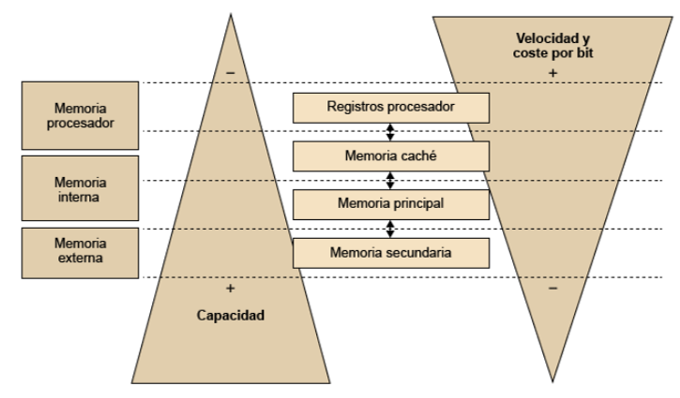
\includegraphics[width=10cm]{Jerarquia.png}
\centering
\caption{Jerarquía de memorias}
\label{fig:Jerarquia}
\end{figure}

\subsubsection{Memoria Caché}
Son dispositivos de capacidad reducida pero de gran velocidad. Se suele encontrar dentro del procesador y están diseñadas para reducir el tiempo de acceso a la memoria. En este dispositivo se almacenan los datos o instrucciones más utilizadas por el procesador. \cite{Estructura}

A su vez se divide en 3 niveles (l1, L2 y L3), el primer nivel está dividido en memoria de instrucciones y memoria de datos. Las últimas dos son unificadas.

\subsubsection{Memoria RAM o principal}
En la memoria principal se almacenan los programas que se deben ejecutar y sus datos, es la memoria visible para el programador mediante su espacio de direcciones.
La memoria principal tiene una capacidad mucho más elevada que la memoria caché (del orden de Gbytes o de Tbytes en supercomputadores). Utiliza tecnología DRAM (Dynamic RAM), que es más lenta que la SRAM, pero con una capacidad de integración mucho más elevada, hecho que permite obtener más capacidad en menos espacio.\cite{Estructura}

\subsubsection{Memoria Virtual}
Es una parte del disco duro designada exclusivamente para soportar partes de programas o datos que están en ejeucción y que el momento no se están ejecutando pero en algún momento lo hará. De esta forma se libera al programador de las restricciones de la memoria principal.

\subsubsection{Memoria Externa}
Esta clasificación corresponde a dispositivos de almacenamiento secundario y también se pueden considerar sistemas de almacenamiento en red. Los dispositivos que forman la memoria externa se conectan al computador con algún tipo de bus (serie o paralelo). Estos dispositivos se pueden encontrar físicamente dentro del computador conectados por buses internos del computador (IDE, SATA, SCSI, etc.) o pueden estar fuera del computador conectados por buses externos (USB, Firewire, eSATA, Infiniband, etc.).\cite{Estructura}



\subsection{Gestión de memoria}

\subsection{Velocidad de memoria}






\section{Conclusiones} \label{conclusion}
XXXX

\bibliographystyle{IEEEtran}
\bibliography{references}

\end{document}
